\section{Results}\label{sec:results}
\begin{framed}
6. Implement and test a part of your system using the ZYBO platform including at least one IP core written and verified with the HLS tool.
\end{framed}

This section shows and elaborates on the results in performance and utilization of all the designs we purposed in section \ref{sec:archdesign}. This includes a high-level synthesis report of the two IP cores (GenerationGenerator and Simulator) and the user application, that was implemented in C++ and deployed to the ZYBO board with the use of OSAPI threads and FreeRTOS. Overall, our results show that simple fixed-point arithmetic can be accelerated in an hardware FPGA at relative low cost, however more complicated floating point computations are better done in software, as the number of required DSP's and lookup tables rapidly increase in such cases.

\subsection{HLS of the GenerationGenerator core}

The IP core was synthesized in C using a VivadoSimulator, a period of 20 and Verilog as the RTL language. Target device is a Zybo model xc7z010clg400-1. We used a SystemC stimuli file to invoke the IP core, which can be found in Appendix A. Figure \ref{fig:ggperformanceestimates} shows the performance estimates of the applied design. We seen that the estimated clock is well within our target of 20 with an uncertainty of 2.50 and the latency lie in range of 0 to 270 where the generateGeneration instance should have one with a latency of 269, and the produceRandom should have one with a latency of 3. It was expected that generateGeneration had a lot higher latency than produceRandom because of the high amount of logic inside it.

\begin{figure}[h!]
	\centering
	\fbox{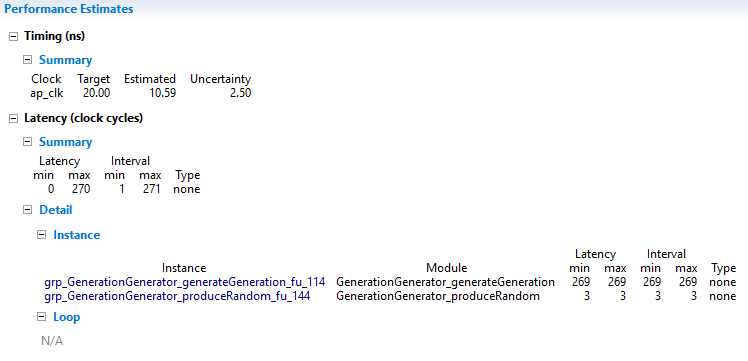
\includegraphics[width=0.9\linewidth]{../diagrams/GGperformanceEstimates.png}}
	\caption{Performance estimation of GenerateGeneration.}
	\label{fig:ggperformanceestimates}
\end{figure}

Figure \ref{fig:ggutilizationestimates} shows utilization of hardware estimates. We see that the demand of resources are well within range of what is available on the ZyBo board. The IP core uses only 5\% of the lookup tables and only 3\% of the flip-flops. This means that it would actually be possible to fit the IP core onto the FPGA.
\FloatBarrier

\begin{figure}[h!]
	\centering
	\fbox{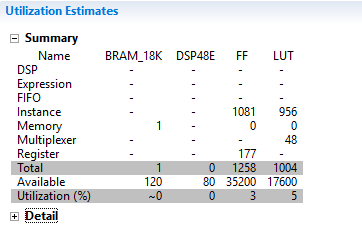
\includegraphics[width=0.6\linewidth]{../diagrams/GGutilizationEstimates.png}}
	\caption{Utilization estimation of GenerateGeneration.}
	\label{fig:ggutilizationestimates}
\end{figure}
\FloatBarrier

Figure \ref{fig:gginterface} shows the generated interface signals. These interfaces are the interfaces, which we specified in the SystemC model. It can be seen that directions are the directions which we specified and the bit width is what we specified in the model.

It should be noted, that most of these ports (all except clk and reset) are accessible through an AXILite interface, which we specified by the use of pragmas. This means, that we are able to communicate with the IP core directly from software through a memory mapped interface.

\begin{figure}[h!]
	\centering
	\fbox{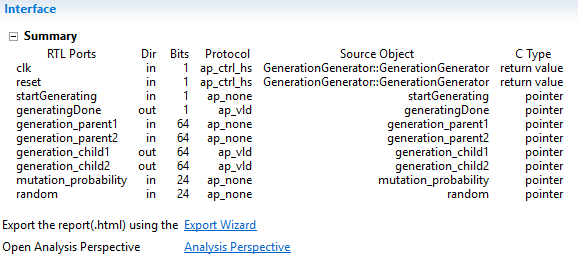
\includegraphics[width=0.8\linewidth]{../diagrams/GGinterface}}
	\caption{Interfaces of GenerateGeneration}
	\label{fig:gginterface}
\end{figure}

Figure \ref{fig:generationgeneratortrace} shows the trace output after running a C simulation with a stimuli, which can be seen in listing \ref{lst:generationGeneratiorStim}. We can seen that the random input data changes continuously, and when the generating core is started, it uses the two parents and a mutation probability to create new children chromosomes and output these. This simulation shows, that the IP core should has the right behaviour. Unfortunately we were not able to run the C/RTL co-simulation  due to a tool issues.

\begin{figure}[h!]
	\centering
	\fbox{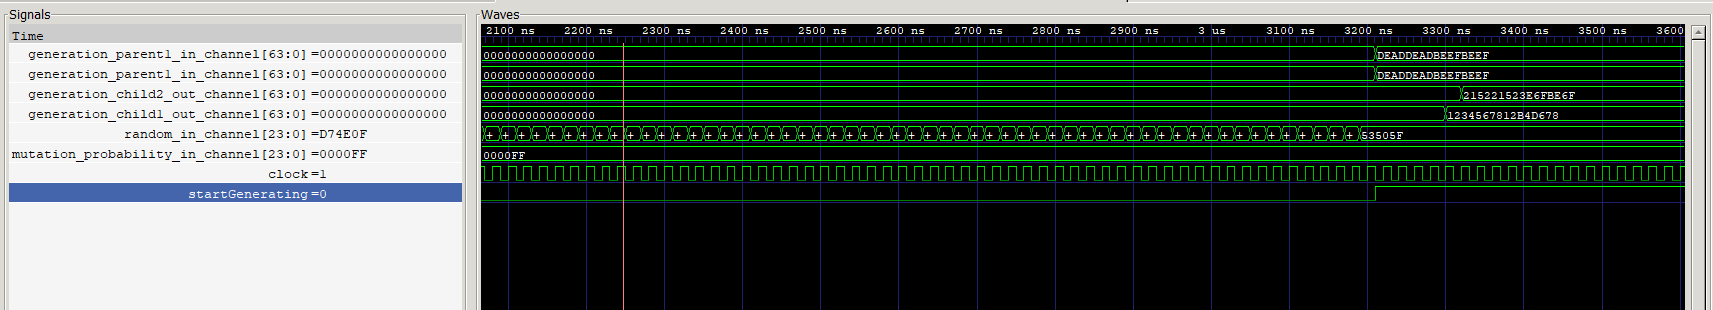
\includegraphics[width=\linewidth]{../diagrams/GenerationGeneratorSim.png}}
	\caption{A trace diagram that shows all bidirectional signals of the module during a example stimulation.}
	\label{fig:generationgeneratortrace}
\end{figure}
\FloatBarrier

\subsection{HLS of the Simulator core}

The IP was synthesized with the same settings as the GenerationGenerator in the Vivado HLS tool. We used a SystemC stimuli file to make calls to the IP core, which can be found in Appendix A. Figure \ref{fig:simperformanceestimates} shows performance estimates, with the estimated clock being within the range of the target clock, though only barely, and the latency being from  0 to 96. The simulateRosenbrock instance should have a latency of between 46 and 95. 

\begin{figure}[h!]
	\centering
	\fbox{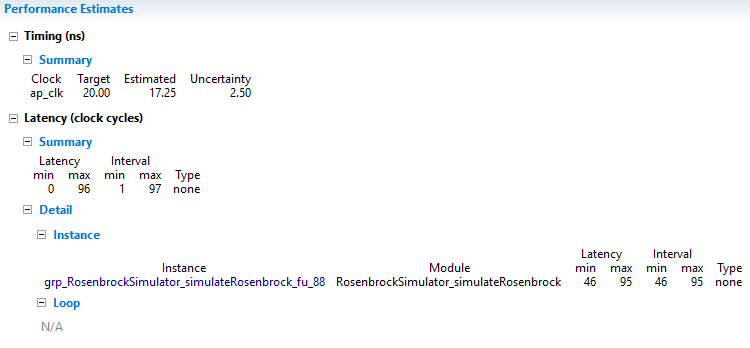
\includegraphics[width=0.7\linewidth]{../diagrams/SimperformanceEstimates.png}}
	\caption{Performance estimation of Simulator}
	\label{fig:simperformanceestimates}
\end{figure}
\FloatBarrier

In figure \ref{fig:ggutilizationestimates} we see the utilization estimates of running the Simulator in hardware. The total resource demand exceed those of the platform, the ZyBo board, by quite a significant margin. 

The algorithm need 592 DSP48E's, but only 80 are available, which means that it needs over 7 times as many as are present on the FPGA. Likewise it needs 39988 flip-flops and 22918 lookup tables, but fewer are available. The flip-flops is only over-utilized by 13\% while the lookup-tables exceeds the available ones by 30\%. 

This means that the current implementation will not be runnable on hardware. We could either use a bigger FPGA or reimplement the design to use another floating point encoding.

\begin{figure}[h!]
	\centering
	\fbox{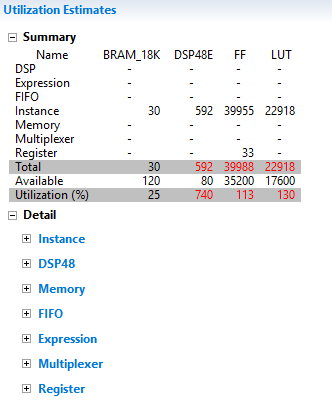
\includegraphics[width=0.6\linewidth]{../diagrams/SimutilizationEstimates.png}}
	\caption{Utilization estimation of Simulator}
	\label{fig:simutilizationestimates}
\end{figure}

Figure \ref{fig:siminterface} shows the generated interfaces. It can be seen that all of the interfaces are as we defined in the SystemC model. These have the bit width as we defined. It should be noted that all except the clk and reset ports will be exported as AXILite memory mapped interfaces. This means that we, if the design would fit on the FPGA, could communicate directly with the IP core from the software.

\begin{figure}[h!]
	\centering
	\fbox{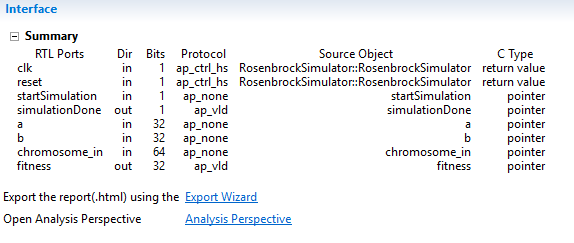
\includegraphics[width=0.7\linewidth]{../diagrams/Siminterface}}
	\caption{Interfaces of GenerateGeneration}
	\label{fig:siminterface}
\end{figure}

\subsection{C++ application}


